%Before characterizing a fiber several tasks had to be performed to check that the system is working properly. The quality of the tightness to the light of the black box used and the correct operation of the PMT for this study, which involves checking the correct operation of the PCB designed and checking the linearity of the PMT output signal in the study range, must be verified.

Before characterizing a fiber several tasks had to be performed to check that the black box is light-tight enough and to check that the PMT response is linear in the studied range of photons intensities.

%First, the quality of the light tightness of the black box used was verified. It is important because we are detecting small signals, a few hundred photons per nanosecond, so it must be verified that the background of the system are below that.

A light leak in the dark box would produce a background larger than the signal. To check the light-tightness of the dark box, the PMT dark current were measured before and after covering the setup using a special black blanket from Thorlabs \cite{BlackBlancket}, that prevents external photons from entering the system. No statistically significant differences were observed between covered and uncovered setup, which indicates the black box is sufficiently light tight. 

%The LED was fed with four different intensities ($0.05~\milli\ampere$, $0.1~\milli\ampere$, $0.15~\milli\ampere$ and $0.2~\milli\ampere$) and the PMT response was measured with and without a special black blanket from Thorlabs \cite{BlackBlancket}, that prevents external photons to reach the system. This test was repeated for three different fibers and the mean and standard deviation of the light output were calculated.

%\begin{equation}
%\bar{x}=\frac{\sum_{i=0}^{N}x_i}{N}; \qquad \sigma = \frac{\sqrt{\sum_{i=0}^{N}(x_i-\bar{x})^2}}{N-1};
%\label{eq:MeanAndStandardDesviation}
%\end{equation}

%The difference of the PMT responses in both cases is plotted in Figure \ref{fig:LightTightnessTest} as a function of the LED intensity. As it can be seen in this figure, there are no statistically relevant differences between covered and uncovered fibers. Therefore, the light tightness of the black box is sufficient for this study.


%\begin{figure}[]
 %\centering
  %\subfloat[The measurement obtained by covering the setup with a special black blanket and not covering.]{
   %\label{subfig:LightTightnessTestData}
    %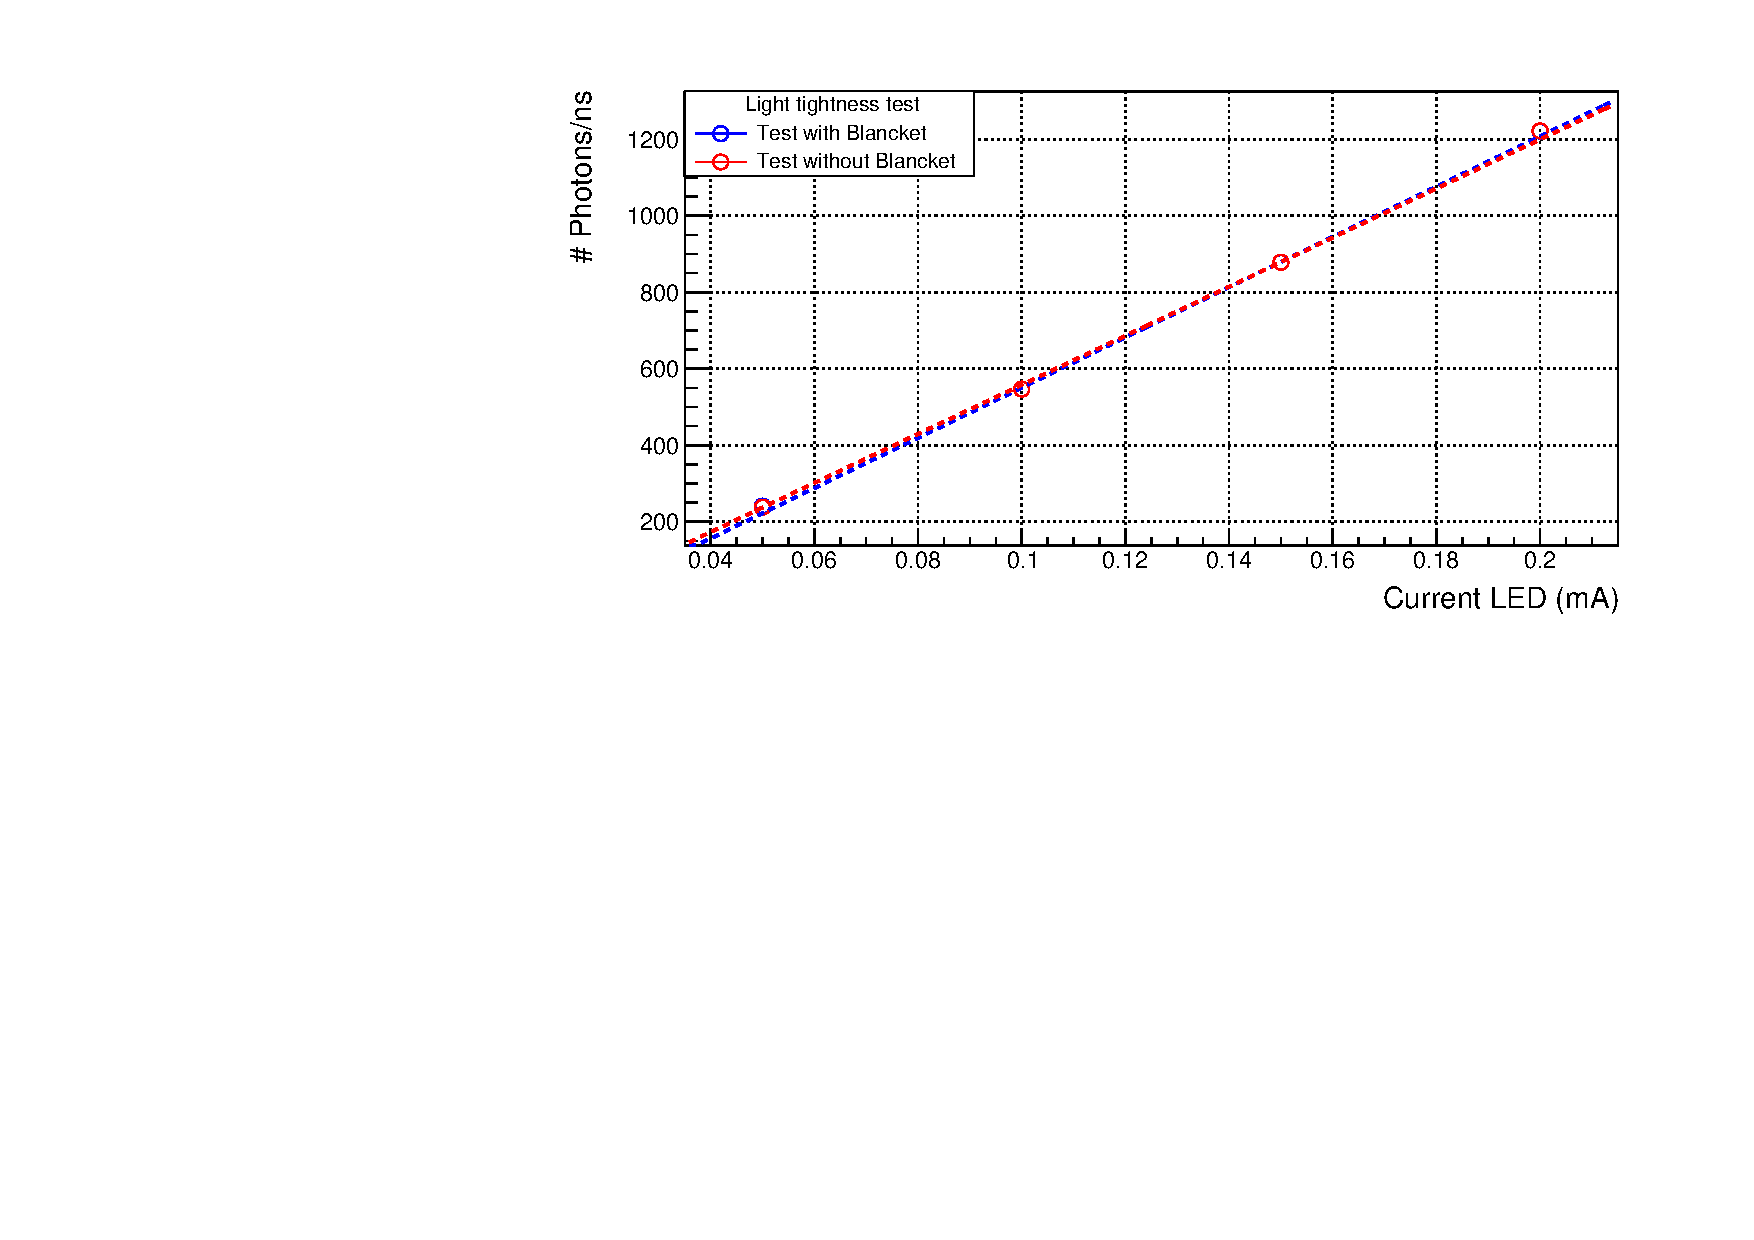
\includegraphics[width=0.9\textwidth]{4ResearchAndDevelopments/41Fibers/Light_tightness_Measurements.pdf}}
    %\newline
  %\subfloat[.]{
   %\label{subfig:LightTightnessTestDifference}
    %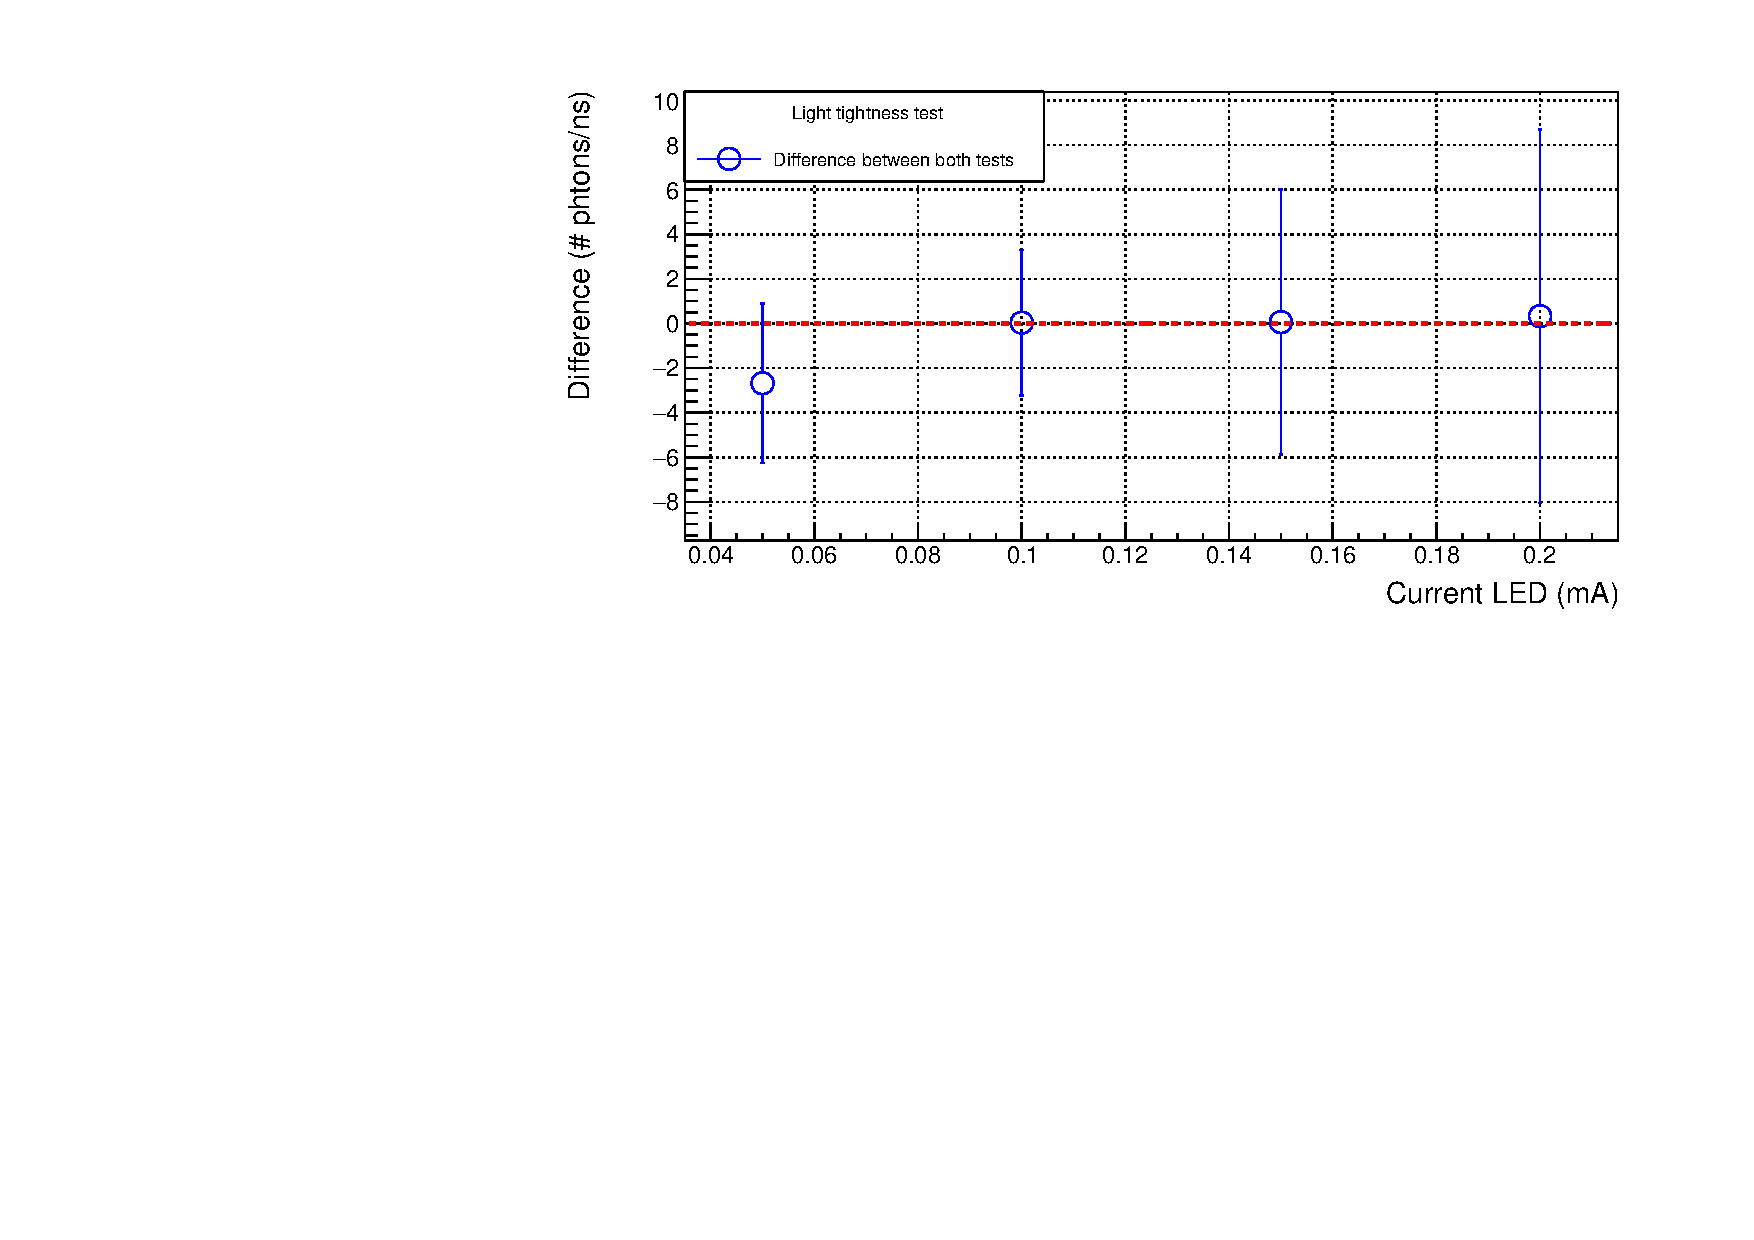
\includegraphics[width=0.9\textwidth]{4ResearchAndDevelopments/41Fibers/Light_tightness_difference.pdf}}
 %\caption{Energy spectrums used to test the effect of the Polishing machine}
 %\label{fig:LightTightnessTest}
%\end{figure}

%\begin{figure}[h]
%\centering
%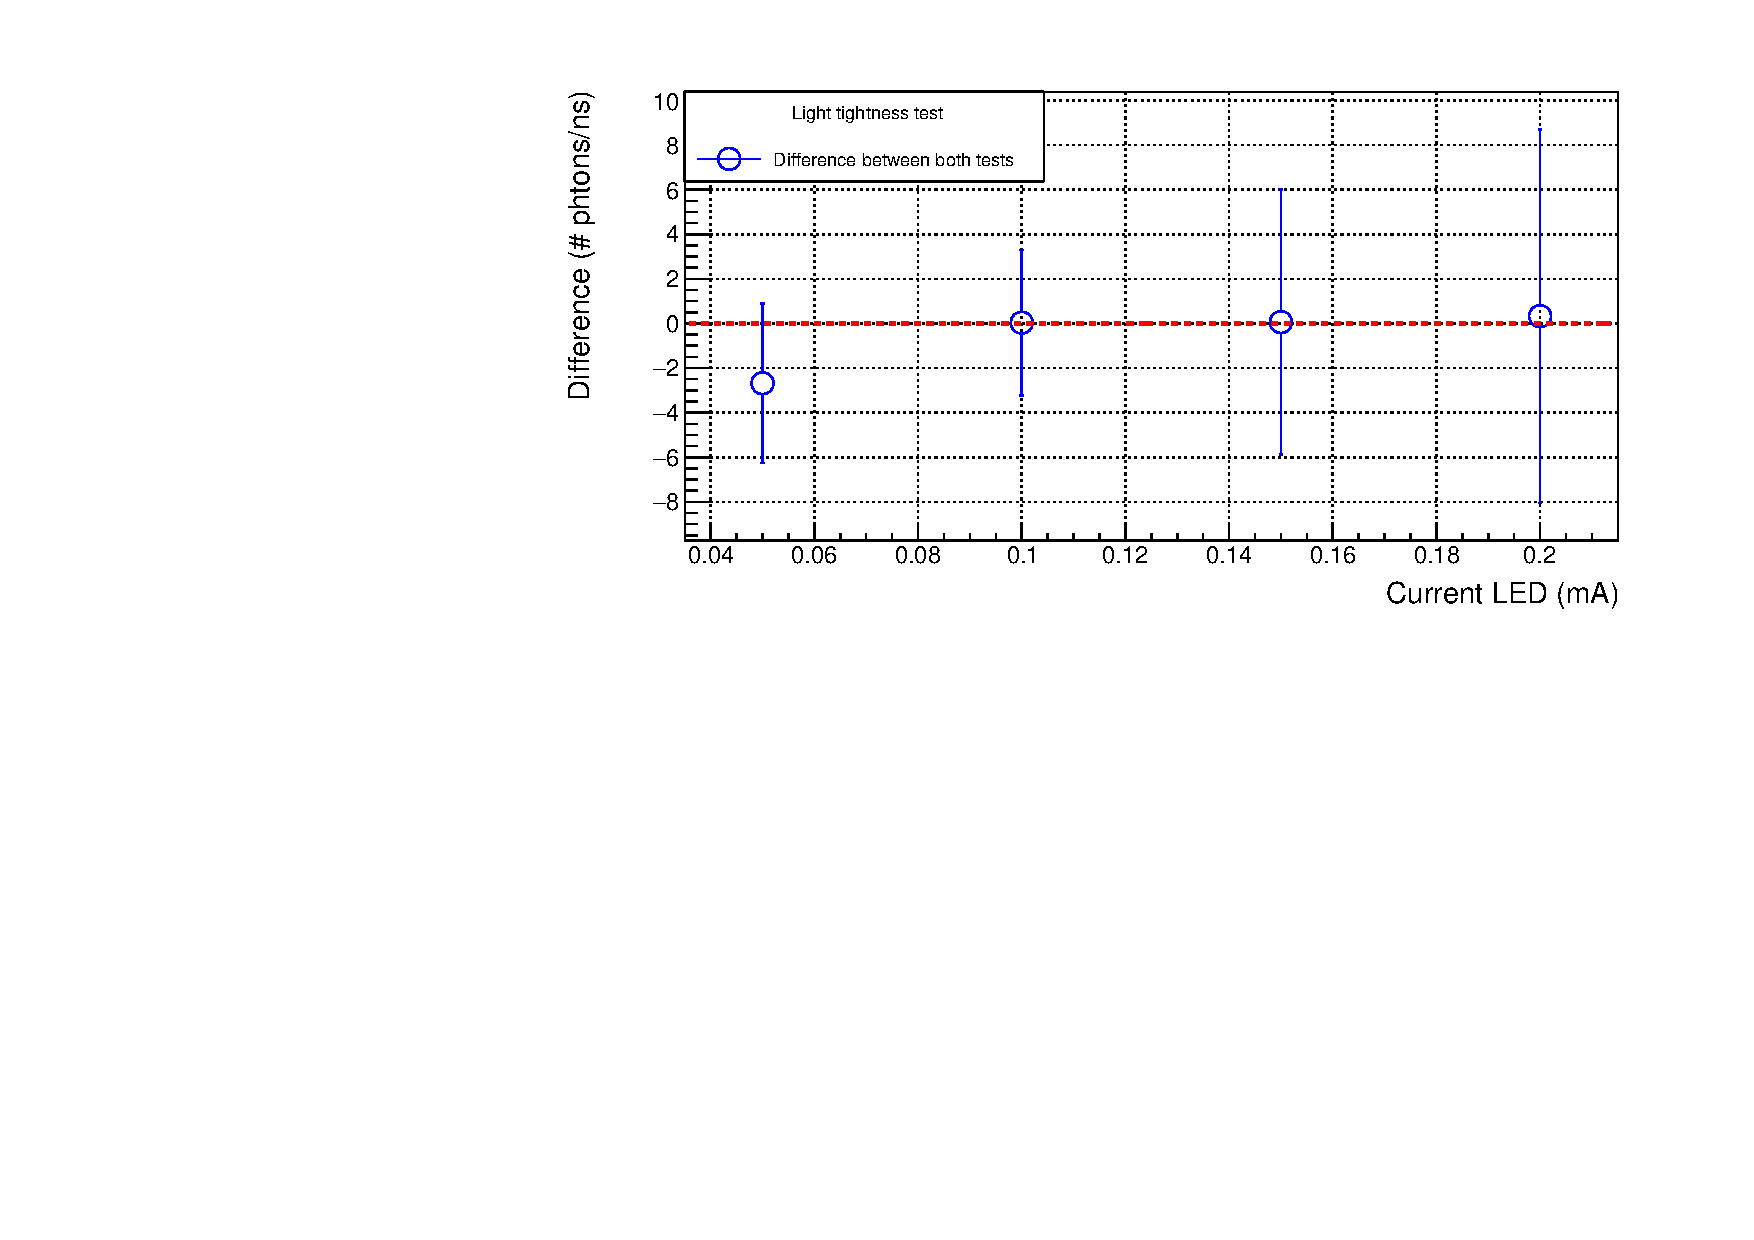
\includegraphics[scale=0.6]{4ResearchAndDevelopments/41Fibers/Light_tightness_difference.pdf}
%\caption{Difference between the results obtained in both tests carried out to check the light-tight quality of the system.\label{fig:LightTightnessTest}}
%\end{figure}

The optimal voltage supply to the PMT was obtained by finding the voltage plateau at which the electron collection efficiency in the first dynode was practically $100\%$ ($CE=1$ in equation \ref{eq:NumPhotonsFromIntensityPMT}). In absence of fibers, the PMT output current was measured for different PMT supply voltages, between $0$ and $500~\volt$, first with the LED OFF (PMT dark current) and then with the LED feed at $1~\milli\ampere$. The number of photons detected by the PMT (difference between both spectra) is plotted in Figure \ref{fig:PlateauNoGainPMT}. As it can be seen, the plateau starts at voltages higher than $150~\volt$. The chosen voltage for the characterization was $250~\volt$.

\begin{figure}[h]
\centering
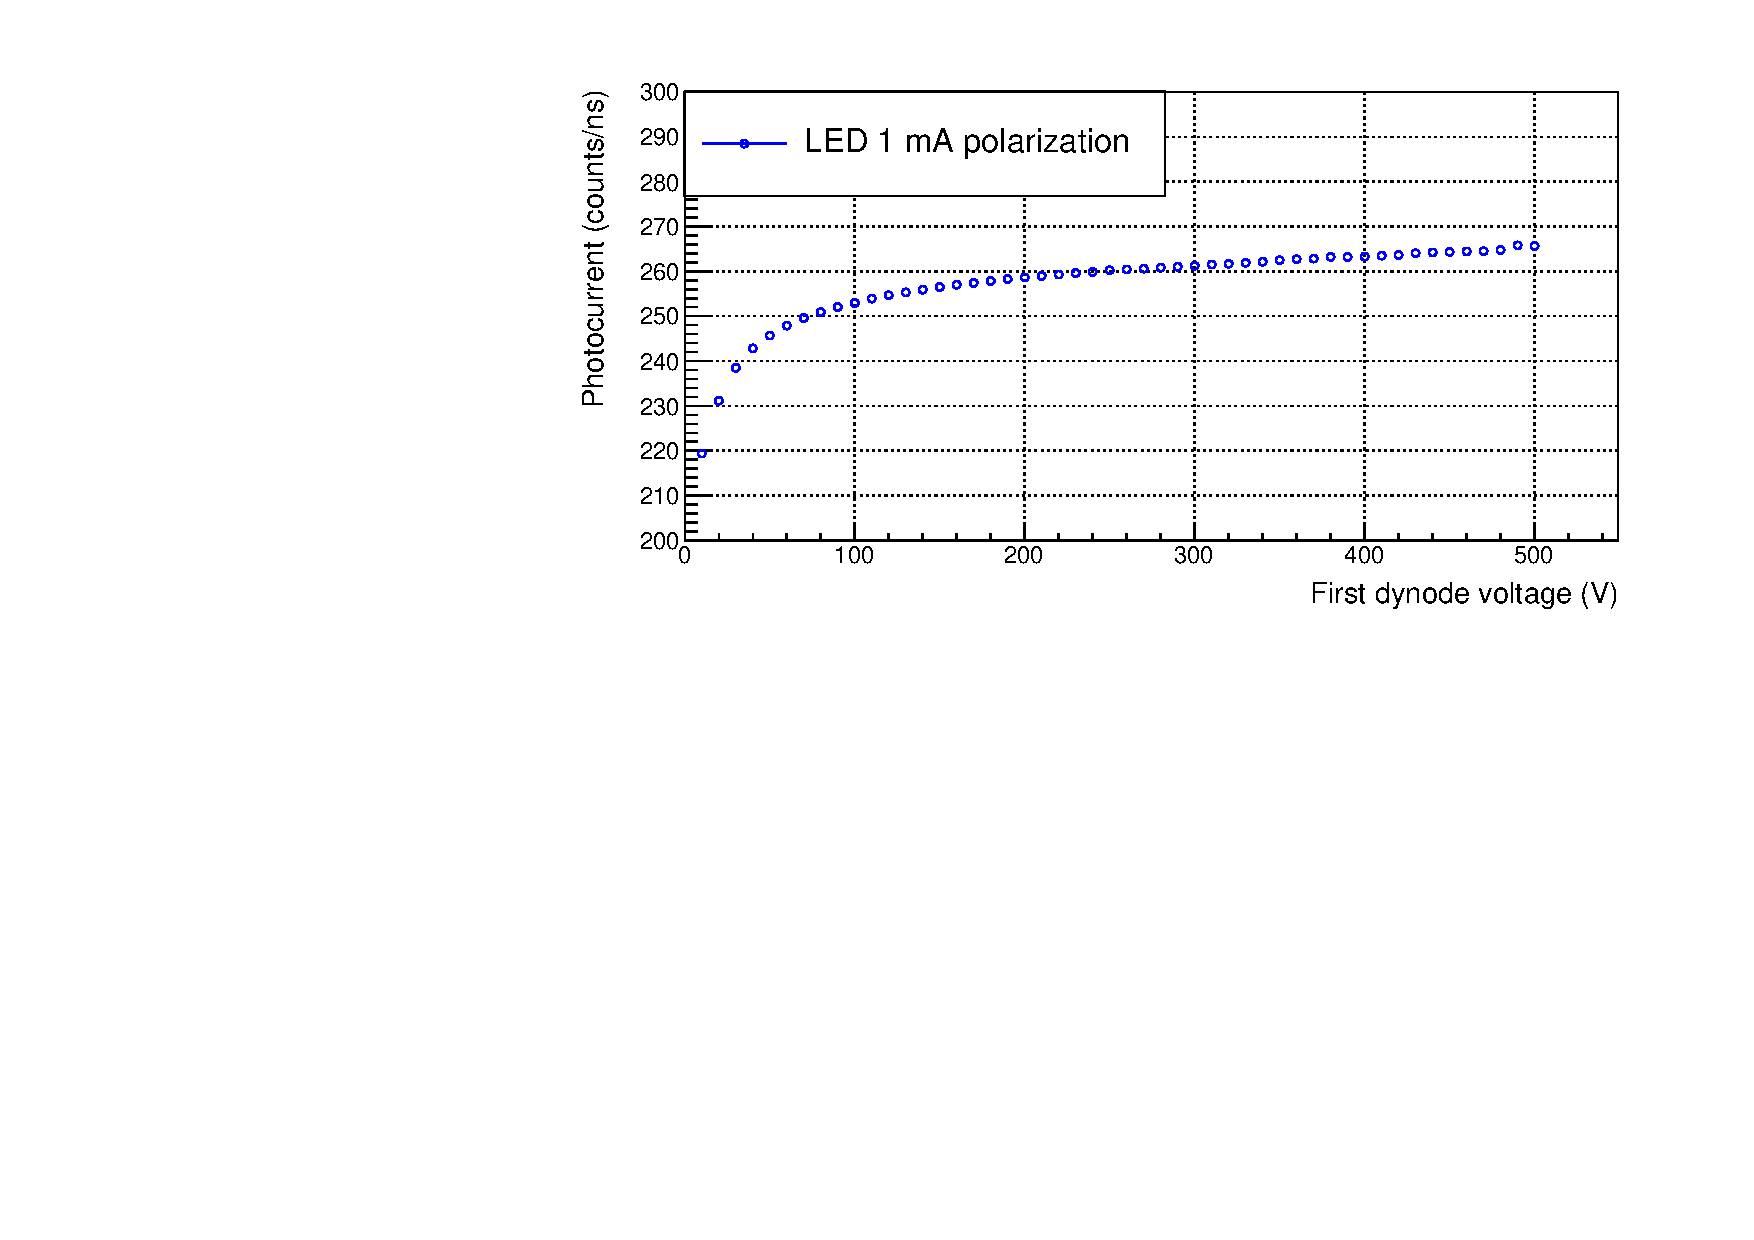
\includegraphics[scale=0.7]{4ResearchAndDevelopments/41Fibers/PCBNoGainPlateau_Calibrated.pdf}
\caption{PMT photocurrent as a function of the first dynode voltage. Error bars are included but they are too small to be visible.\label{fig:PlateauNoGainPMT}}
\end{figure}

Finally, the linear response of the PMT was verified. The LED was powered in current mode with intensities ranging from 0 to $10~\milli\ampere$, the linearity of which was previously tested in the laboratory. This was tested in the range of the number of photons expected for a tritium event (a few tens of photons per tritium event, which gives tens of photons per nanosecond) and in a broader range, around two thousand five hundred photons per nanosecond, interesting in the case of higher tritium activities. The linearity test was performed without fibers coupled to the PMT. Several collimators were used to reduce the amount of photons that reach the PMT. The results in low and high illumination cases are shown in Figures \ref{fig:LinearityRangesOfPMT}. As it can be seen, no saturation in the PMT response is observed.

\begin{figure}
\centering
    \begin{subfigure}[b]{1\textwidth}
    \centering
    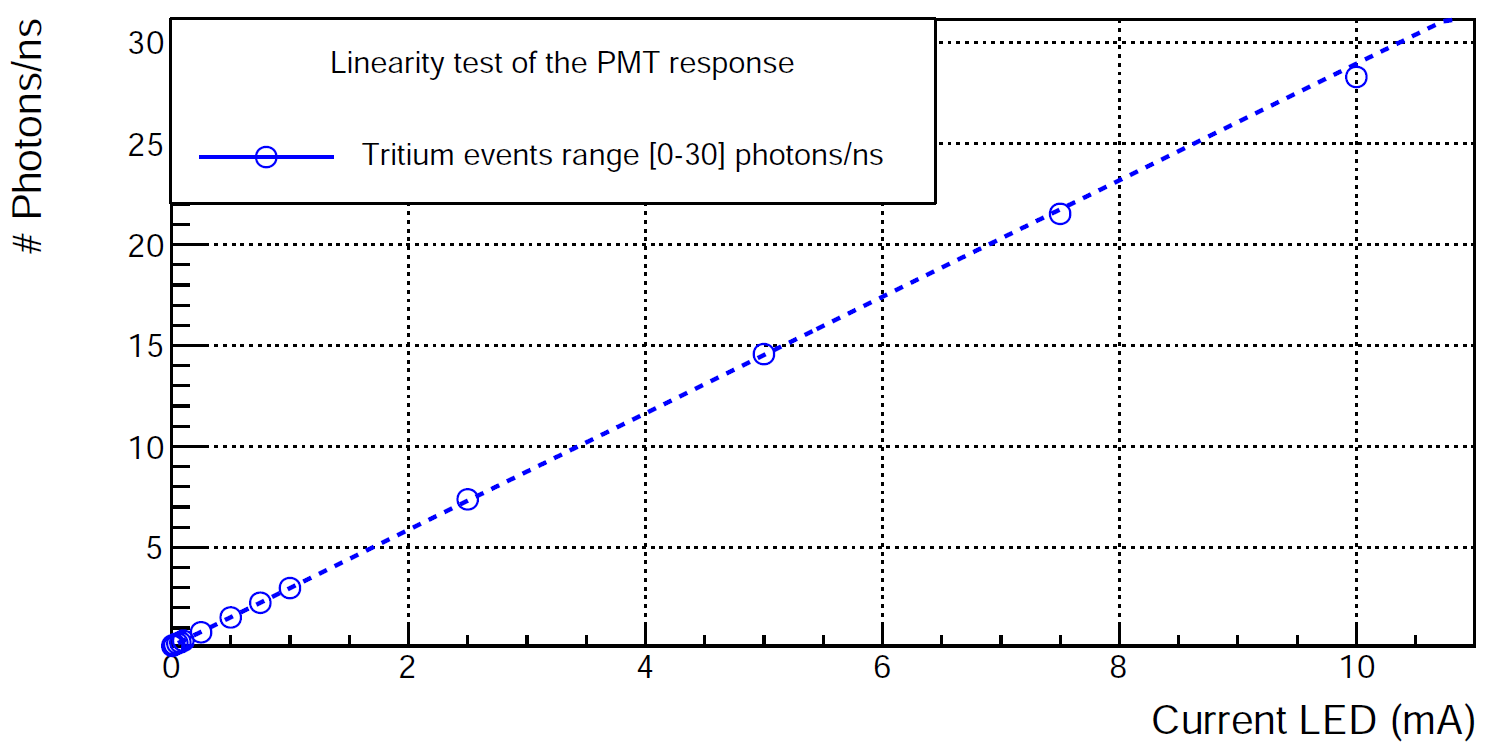
\includegraphics[scale=0.4,width=\textwidth]{4ResearchAndDevelopments/41Fibers/Linearity_test_0_30_range.png}  
    \caption{\label{subfig:LinearityTritiumRange}}
    \end{subfigure}
    \hfill
    \begin{subfigure}[b]{1\textwidth}
    \centering
    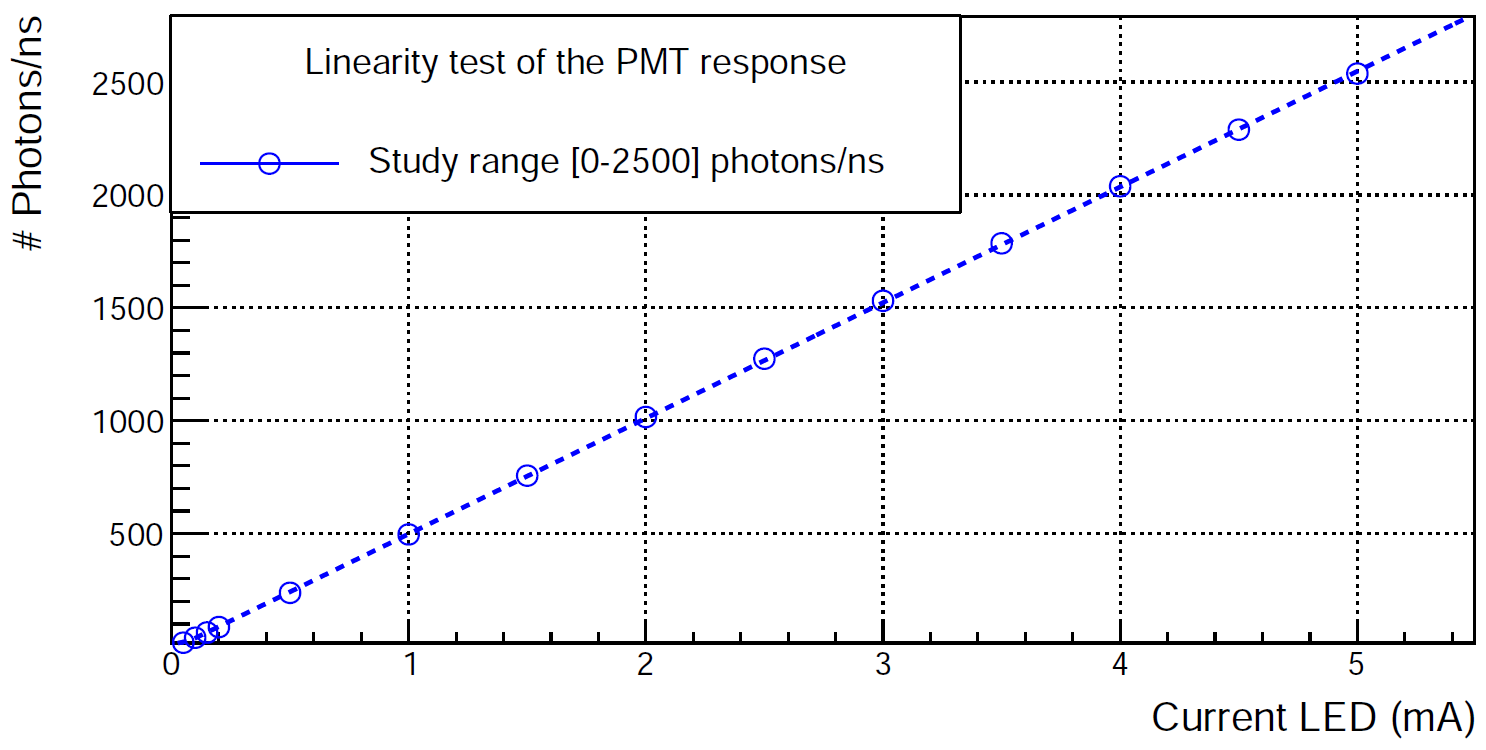
\includegraphics[scale=0.4, width=\textwidth]{4ResearchAndDevelopments/41Fibers/Linearity_test_0_2500_range.png}  
    \caption{\label{subfig:LinearityStudyRange}}
    \end{subfigure}
 \caption{Number of photons measured by the PMT as a function of the polarization current of the LED. a) Response of the PMT in the intensity range of tritium events. b) Response of the PMT in the range $0-2500~\text{photons}/\nano\second$. Error bars are included but they are too small to be visible.}
 \label{fig:LinearityRangesOfPMT}
\end{figure}